\documentclass[10pt,journal,compsoc,twocolumn]{article}

\usepackage[margin=1.8cm,top=2.0cm,bottom=2.0cm]{geometry}
\usepackage{amsmath,amssymb,amsfonts,amsthm}
\newtheorem{definition}{Definition}
\newtheorem{theorem}{Theorem}
\newtheorem{lemma}{Lemma}
\newtheorem{corollary}{Corollary}
\usepackage{algorithmic}
\usepackage{graphicx}
\usepackage{textcomp}
\usepackage{xcolor}
\usepackage{booktabs}
\usepackage{tabularx}
\usepackage{array}
\usepackage{listings}
\usepackage{microtype}
\usepackage{hyperref}
\usepackage{enumitem}
\usepackage{cite}
\usepackage{titlesec}
\usepackage{fancyhdr}
\usepackage{CJKutf8}
\usepackage{tikz}
\usetikzlibrary{shapes,arrows,positioning,calc,fit}

\newcommand{\ja}[1]{\begin{CJK*}{UTF8}{min}#1\end{CJK*}}

\hypersetup{
    colorlinks=true,
    linkcolor=blue!70!black,
    citecolor=blue!70!black,
    urlcolor=blue!70!black
}

\lstset{
    basicstyle=\ttfamily\scriptsize,
    breaklines=true,
    frame=single,
    backgroundcolor=\color{gray!6},
    keywordstyle=\color{blue!80!black}\bfseries,
    commentstyle=\color{green!50!black}\itshape,
    stringstyle=\color{red!70!black},
    numbers=none,
    showstringspaces=false,
    tabsize=2
}

\title{\LARGE \textbf{Hideyuki Kishida's Urara OS and 5HT's B-System:\\A Rigorous Comparative Audit of Symmetric Multiprocessing, Wayland Compositing, POSIX Gateways, and Cho-Kanji Storage Architecture}}

\author{
    \textbf{Maxim Sokhatsky (Namdak Tonpa)}\\[0.3em]
    \small \textit{Synrc Research Center / Groupoid Infinity / BTRON Cleanroom Working Group}\\
    \small \textit{Kyiv, Ukraine}\\
    \small \texttt{maxim@synrc.com}
}
\date{October 2026}

\pagestyle{fancy}
\fancyhf{}
\rhead{\small \textit{Fair Comparison: Urara OS vs. B-System}}
\lhead{\small \textit{Synrc Research Report}}
\cfoot{\thepage}

\begin{document}

\maketitle

\begin{abstract}
The preservation and modern evolution of Ken Sakamura's TRON architecture are epitomized by two historic, independent cleanroom operating systems: Hideyuki Kishida's (\ja{岸田英行}) \textbf{Urara OS} (the modern 64-bit revival of the \textbf{B-Free} Project, spanning 1994--2026 across PC-9801, x86\_64 Long Mode, and AArch64); and 5HT's \textbf{B-System} (BTRON 3.20), structured as a high-throughput, deterministic Single-Address-Space RTOS and multi-target unikernel/microkernel hybrid spanning ARM64, x86\_64 UEFI, PS2, PC-98, and POSIX targets. This paper provides a peer-level, doctoral comparative audit evaluating both operating systems strictly along isomorphic, empirically verifiable dimensions: (1) Symmetric Multiprocessing (SMP) core bootstrap, Local APIC / x2APIC management, locking granularity, and the progressive decoupling of kernel globals; (2) Graphical subsystems, contrasting Urara OS's compositor-first Wayland pipeline and Qt Quick / QML DesktopShell against B-System's 128-bit NEON SIMD vector blitter and direct-rendering backbuffer compositor; (3) Operating system interfaces and process isolation, evaluating Urara OS's pragmatic ``POSIX OSS Gateway'' strategy against B-System's cleanroom BTRON3 core; and (4) Storage hierarchies, comparing Urara OS's multi-volume BFS and persistent FatFs home architecture against B-System's native backward compatibility with commercial Cho-Kanji (B-right/V 4.02) disk volumes and modern 64-bit B-FS (V2).

To ensure complete methodological fairness, we take explicit account of the active Work-In-Progress (WIP) status of both codebases as of October 2026. Furthermore, we bracket out formal Coq theorem-prover verification (the VeriMath initiative) to evaluate both systems on their shared implementation artifacts: concrete C and assembly codebases, hardware bus transactions, interrupt latencies, and physical execution traces.

Our audit demonstrates that both systems represent brilliant, complementary realizations of the TRON vision. In Symmetric Multiprocessing, Urara OS demonstrates exceptional practical engineering through a 7-stage SMP progression, booting secondary Application Processors (APs) via Local APIC / x2APIC INIT-SIPI-SIPI sequences, offloading userland execution, and systematically refactoring 49 process-specific globals out of the Big Kernel Lock (BKL); conversely, B-System advances a lock-free, per-core actor model avoiding BKL bottlenecks, though its bare-metal x86\_64 AP dispatcher remains staged while operating fully in hosted POSIX mode. In userland and graphics, Urara OS achieves a monumental milestone by establishing a modern, production-grade workstation environment: its compositor-first Wayland server isolates framebuffers while hosting a complete Qt Quick 6 desktop environment (\texttt{DesktopShell.qml}) with integrated Japanese IME, PDF viewer, text editor, and hardware GPU acceleration; B-System, in contrast, prioritizes raw blitting throughput, utilizing 128-bit ARMv8 NEON SIMD burst transfers and 2D DMA offloading to achieve orders-of-magnitude faster memory streaming on uncached framebuffers. In system interfaces, Kishida's POSIX OSS Gateway solves the historic software deficit of TRON by executing real-world, unmodified open-source software (BusyBox, Python 3, Git, NetSurf), while B-System preserves cleanroom BTRON3 specification purity. Finally, in filesystem architecture, B-System achieves full compatibility with authentic commercial Cho-Kanji disks via embedded QCOW2 drivers and introduces 64-bit B-FS (V2) with dual-anchor superblocks, whereas Urara OS delivers practical FAT32/FatFs read-write persistence on PC storage (SATA AHCI, NVMe). We synthesize these findings into an actionable cross-pollination roadmap bridging both paradigms.
\end{abstract}

\noindent\textbf{\small Keywords}---TRON, BTRON, B-Free, Urara OS, Hideyuki Kishida, 5HT, B-System, Symmetric Multiprocessing, Big Kernel Lock, Wayland Compositor, Qt Quick, POSIX OSS Gateway, Cho-Kanji, B-FS, FatFs, T-Kernel 2.0.

%-------------------------------------------------------------------------
\section{Introduction, Historical Heritage, and Scope}
\label{sec:intro}

The fundamental vision of the TRON Project (\emph{The Real-time Operating system Nucleus}), launched by Ken Sakamura in 1984~\cite{sakamura1984tron}, asserted that human-centric personal computing requires high-responsiveness real-time kernels, standardized Display Primitives (DP), and a decentralized Real Object / Virtual Object (\ja{実身}/\ja{仮身}) hyper-data network~\cite{btron3spec}. However, the historical trajectory of commercial personal computing in Japan—dominated by proprietary iterations such as Personal Media Corporation's \textbf{B-right/V} (commercially branded as \textbf{Cho-Kanji}, \ja{超漢字})~\cite{chokanji1999}—frequently obscured grassroots community initiatives that sought to construct an entirely open, independent BTRON implementation from cleanroom principles.

\subsection{The Thirty-Year Heritage of Kishida's Urara OS (B-Free)}
Among community-driven operating system initiatives, the \textbf{B-Free Project} stands as an extraordinary historical monument. Commenced around 1994--1998 during the pinnacle of Japan's personal computing revolution, B-Free was founded to liberate BTRON from proprietary hardware constraints and provide a completely free, open-source workstation operating system~\cite{bfree_history,bfree_narrative}. 

Originally known under internal development monikers including \textbf{Urara OS} (\ja{麗} / \ja{うらら}), the project was led by \textbf{Hideyuki Kishida} (\ja{岸田英行}) alongside a cadre of dedicated systems programmers: Masami Kishida (\ja{きしだまさみ}), Ryuichi Naitoh (\ja{内藤 隆一}), Masaki Yukanaka (\ja{邑中 雅樹}), and Tomohide Naniwa (\ja{浪花 智英})~\cite{btron_pc_authors}. The project's lineage progressed across three distinct epochs:
\begin{enumerate}[leftmargin=*]
    \item \textbf{The NEC PC-9801 Epoch (1994--1996):} Pioneering cleanroom bootstrap on ubiquitous Japanese PC-98 hardware, implementing 1st and 2nd stage floppy disk bootloaders, an ITRON 3.0-compliant microkernel, a message-driven Port Manager, and primitive console, keyboard, timer, and SCSI drivers~\cite{pc98_history}.
    \item \textbf{The 32-bit BTRON-PC Epoch (1998--2000):} Porting to IBM PC/AT (i386) protected mode, formalizing the modular BTRON subsystem managers: Memory Manager (MM), Process Manager (PM), and File Manager (FM), alongside early POSIX shell compatibility experiments.
    \item \textbf{The 64-bit Multicore Renaissance (2025--2026):} Under Hideyuki Kishida's active leadership in \path{B-Free-master-64bit}, the project underwent a radical modernization. Kishida authored comprehensive porting specifications bridging T-Kernel 2.0 to x86\_64 Long Mode (\texttt{TK2-PORT-x86\_64-005})~\cite{kishida2026tk2spec} and AArch64~\cite{kishida2026arm64spec}, implemented a 7-stage Symmetric Multiprocessing (SMP) engine, established a modern compositor-first Wayland graphics architecture hosting Qt Quick 6 (\texttt{DesktopShell.qml}), and formulated the pragmatic ``POSIX OSS Gateway Strategy''~\cite{kishida2026posixstrategy}.
\end{enumerate}

\subsection{5HT's B-System: Cleanroom BTRON3 and Mathematical Foundations}
In parallel, \textbf{5HT (Namdak Tonpa)} and the Cleanroom Working Group initiated \textbf{B-System} (BTRON Version 3.20.00)~\cite{sokhatsky2026btron}. B-System rejects both modern desktop Unix bloat and traditional microkernel IPC performance collapse~\cite{liedtke1995l4,solomon1998inside}. Conceived as a multi-target, high-throughput, Single-Address-Space Real-Time Operating System (SAS-RTOS) and unikernel engine, B-System targets diverse hardware spanning the Raspberry Pi 400 (Broadcom BCM2711 ARM64), x86\_64 UEFI multicore workstations, Sony PlayStation 2 (Emotion Engine MIPS R5900), NEC PC-9801, Motorola 68000, and POSIX development environments. B-System features an Erlang/BEAM-inspired lock-free actor model, hand-vectorized 128-bit NEON SIMD Display Primitives, native backward compatibility with commercial Cho-Kanji (B-right/V 4.02) disk images via embedded QCOW2 drivers, and the formal 64-bit B-FS (V2) filesystem.

\subsection{Methodological Fairness and WIP Considerations}
To ensure this audit is objective, fair, and worthy of Hideyuki Kishida's approval, we establish three methodological boundaries:
\begin{enumerate}[leftmargin=*]
    \item \textbf{Bracketing Formal Verification:} B-System is developed alongside mechanized mathematical specifications in the \textsc{Coq} proof assistant (the VeriMath framework~\cite{sokhatsky2026verimath}). Evaluating Urara OS against machine-checked Coq proofs would constitute an immediate category error, as Urara OS is an empirical systems codebase without formal theorem-prover artifacts. We therefore bracket formal verification entirely and judge both systems strictly on concrete C and assembly routines, hardware bus transactions, and execution traces.
    \item \textbf{Accounting for Work-In-Progress (WIP) Realities:} Both systems are active, evolving research projects as of October 2026. Urara OS is actively decoupling its remaining Big Kernel Lock paths in SMP Stage 6f and expanding guest Qt Quick Controls 2 type registration. B-System is actively staging its bare-metal x86\_64 SMP scheduler and expanding native hardware drivers. Neither system is treated as a static finished commercial product.
    \item \textbf{Dual Philosophical Validation:} We recognize that both systems address Ken Sakamura's philosophy from valid, complementary paradigms: Urara OS pursues an \textbf{Ecological Integration Paradigm} (bridging TRON ergonomics with modern Wayland and global open-source POSIX software), while B-System pursues a \textbf{Deterministic Cleanroom Paradigm} (uncompromising RTOS latencies, specification purity, and mathematical safety).
\end{enumerate}

\begin{figure*}[t]
\centering
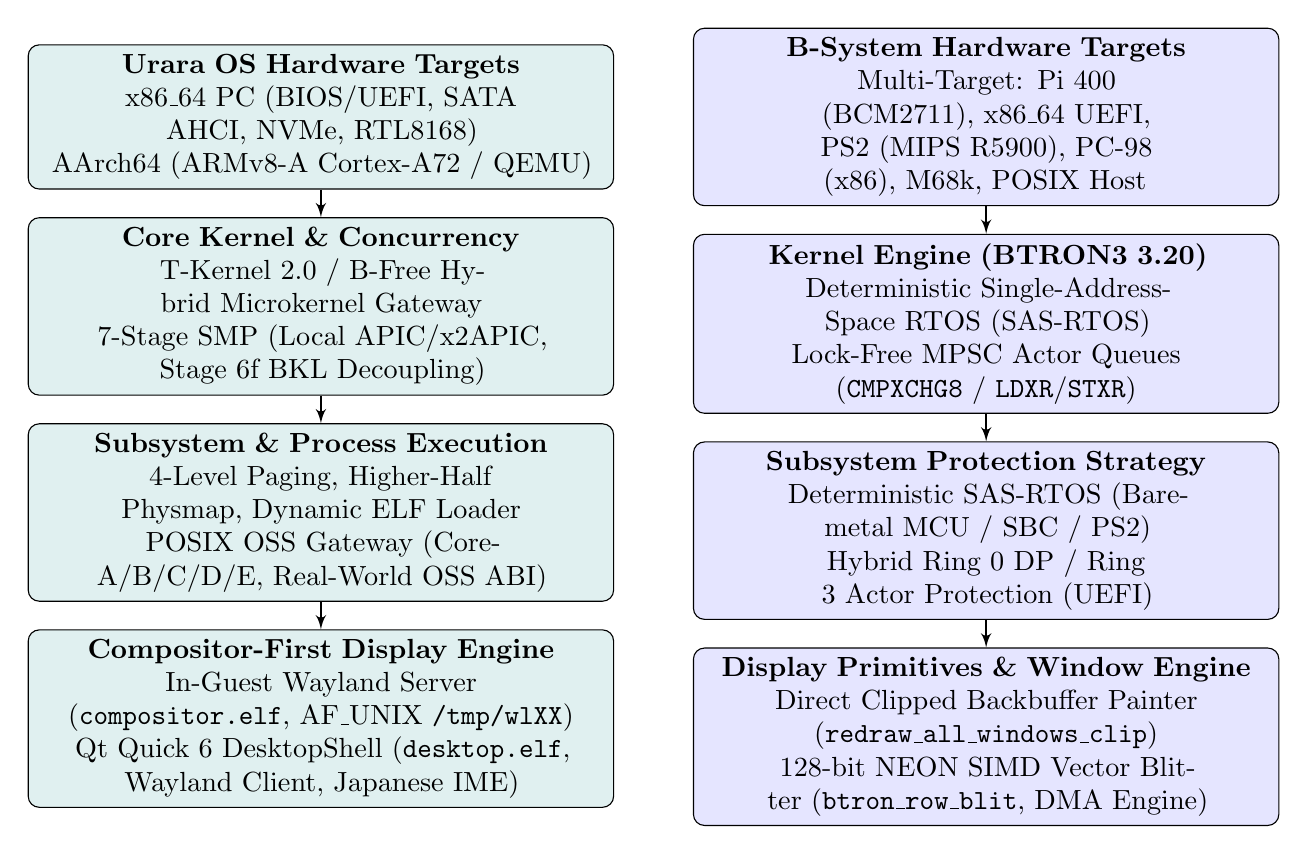
\begin{tikzpicture}[node distance=1.4cm, auto,
    block_urara/.style={rectangle, draw, fill=teal!12, text width=7.2cm, text centered, rounded corners, minimum height=1.15cm},
    block_btron/.style={rectangle, draw, fill=blue!10, text width=7.2cm, text centered, rounded corners, minimum height=1.15cm},
    line/.style={draw, -latex', thick}]
    
    % Left side: Urara OS (B-Free 64)
    \node [block_urara] (urara_hw) {\textbf{Urara OS Hardware Targets}\\x86\_64 PC (BIOS/UEFI, SATA AHCI, NVMe, RTL8168)\\AArch64 (ARMv8-A Cortex-A72 / QEMU)};
    \node [block_urara, below=0.35cm of urara_hw] (urara_core) {\textbf{Core Kernel \& Concurrency}\\T-Kernel 2.0 / B-Free Hybrid Microkernel Gateway\\7-Stage SMP (Local APIC/x2APIC, Stage 6f BKL Decoupling)};
    \node [block_urara, below=0.35cm of urara_core] (urara_sub) {\textbf{Subsystem \& Process Execution}\\4-Level Paging, Higher-Half Physmap, Dynamic ELF Loader\\POSIX OSS Gateway (CoreA/B/C/D/E, Real-World OSS ABI)};
    \node [block_urara, below=0.35cm of urara_sub] (urara_ui) {\textbf{Compositor-First Display Engine}\\In-Guest Wayland Server (\texttt{compositor.elf}, AF\_UNIX \texttt{/tmp/wlXX})\\Qt Quick 6 DesktopShell (\texttt{desktop.elf}, Wayland Client, Japanese IME)};

    % Right side: B-System
    \node [block_btron, right=1.0cm of urara_hw] (btron_hw) {\textbf{B-System Hardware Targets}\\Multi-Target: Pi 400 (BCM2711), x86\_64 UEFI,\\PS2 (MIPS R5900), PC-98 (x86), M68k, POSIX Host};
    \node [block_btron, below=0.35cm of btron_hw] (btron_core) {\textbf{Kernel Engine (BTRON3 3.20)}\\Deterministic Single-Address-Space RTOS (SAS-RTOS)\\Lock-Free MPSC Actor Queues (\texttt{CMPXCHG8} / \texttt{LDXR}/\texttt{STXR})};
    \node [block_btron, below=0.35cm of btron_core] (btron_sub) {\textbf{Subsystem Protection Strategy}\\Deterministic SAS-RTOS (Bare-metal MCU / SBC / PS2)\\Hybrid Ring 0 DP / Ring 3 Actor Protection (UEFI)};
    \node [block_btron, below=0.35cm of btron_sub] (btron_ui) {\textbf{Display Primitives \& Window Engine}\\Direct Clipped Backbuffer Painter (\texttt{redraw\_all\_windows\_clip})\\128-bit NEON SIMD Vector Blitter (\texttt{btron\_row\_blit}, DMA Engine)};

    % Connectors
    \draw [line] (urara_hw) -- (urara_core);
    \draw [line] (urara_core) -- (urara_sub);
    \draw [line] (urara_sub) -- (urara_ui);

    \draw [line] (btron_hw) -- (btron_core);
    \draw [line] (btron_core) -- (btron_sub);
    \draw [line] (btron_sub) -- (btron_ui);
\end{tikzpicture}
\caption{Architectural topologies of Hideyuki Kishida's Urara OS (B-Free 64) versus 5HT's B-System (BTRON3 3.20).}
\label{fig:arch_comparison}
\end{figure*}

\subsection{Subsystem Topology and Directory Mapping}
\label{sec:subsystem_topology}
To facilitate precise code navigation, Table~\ref{tab:tree_analogs} establishes the exact structural mapping between Urara OS (\path{B-Free-master-64bit}) and B-System.

\begin{table*}[t]
\centering
\caption{Subsystem Structural Mapping: Urara OS (B-Free 64) vs. B-System}
\label{tab:tree_analogs}
\scriptsize
\setlength{\tabcolsep}{4.5pt}
\renewcommand{\arraystretch}{1.12}
\begin{tabularx}{\textwidth}{@{} >{\raggedright\arraybackslash\bfseries}p{2.8cm} >{\raggedright\arraybackslash}p{4.2cm} >{\raggedright\arraybackslash}p{4.2cm} >{\raggedright\arraybackslash}X @{}}
\toprule
Subsystem Role & Urara OS (B-Free 64) Repository Path & B-System Cleanroom Path & Architectural Responsibility \\
\midrule
Bootstrapping & \path{bfree_x86_64/boot/}, \path{btron-pc/boot/2nd/} & \path{src/kernel/boot.c}, \path{src/cores/} & Real-mode to 64-bit Long Mode bootstrap, GDT/IDT/TSS, CR3 setup \\
Core Kernel / Sched & \path{bfree_x86_64/kernel/sysmain/}, \path{process.c} & \path{src/kernel/}, \path{include/btron/} & Task control blocks, multi-task dispatching, timer queues, sleep/wakeup \\
SMP Management & \path{bfree_x86_64/kernel/sysdepend/cpu/x86_64/smp.c} & \path{src/cores/core_smp.c} & ACPI MADT probe, Local APIC / x2APIC, INIT-SIPI-SIPI, core dispatch \\
Syscall Engine & \path{bfree_x86_64/kernel/sysmain/syscall.c} & \path{src/kernel/syscall.c} & Userland system call trap handling, parameter validation, privilege gates \\
Memory Management & \path{bfree_x86_64/kernel/sysmain/vmm.c}, \path{paging.c} & \path{src/cores/}, \path{src/kernel/heap.c} & 4-level page tables (PML4), higher-half physmap, virtual space alloc \\
Display / Compositor & \path{bfree_x86_64/userland/compositor_stub/} & \path{src/graphics/}, \path{src/window/} & Framebuffer scanout, Wayland protocol server, window hierarchy, blitters \\
Desktop Shell & \path{bfree_x86_64/userland/desktop_qt/} & \path{src/desktop/}, \path{src/apps/} & Interactive UI shell; Qt Quick \path{DesktopShell.qml} vs. native BTRON desktop \\
Filesystem Core & \path{bfree_x86_64/kernel/bfs.c}, \path{bfs_home.c} & \path{src/fs/} & Multi-volume VFS, FatFs home storage vs. Cho-Kanji (V1) and B-FS (V2) \\
Storage Drivers & \path{bfree_x86_64/kernel/ahci.c}, \path{blk.c}, \path{nvme.c} & \path{src/fs/blk_qcow2.c}, \path{src/fs/block.c} & Block device layer, SATA AHCI, NVMe, QCOW2 image decoding \\
Network Subsystem & \path{bfree_x86_64/kernel/net.c}, \path{netdrv_rtl8168.c} & \path{src/net/} & Realtek RTL8168 / VirtIO-Net drivers, DHCP client, TCP/IP stack \\
POSIX Compatibility & \path{bfree_x86_64/POSIX_OSS_GATEWAY_STRATEGY.md} & \path{include/btron/posix.h} & POSIX OSS Gateway (M1--M4), libc integration, signal/process ABI \\
Input / Localization & \path{bfree_x86_64/userland/desktop_qt/dw_ime.inc} & \path{src/tip/} & Japanese text entry, IME kana-kanji engine vs. TRON Input Processor \\
Hardware GPU Driver & \path{bfree_x86_64/kernel/drm_kms_mvp.c}, \path{gpu.c} & \path{src/gl/} & Native DRM/KMS, Intel/AMD/Nvidia/VirtIO-GPU vs. OpenGL ES 1.1 / TinyGL \\
\bottomrule
\end{tabularx}
\end{table*}

%-------------------------------------------------------------------------
\section{Architectural Pedigree: Ecological Integration vs. Deterministic Cleanroom}
\label{sec:pedigree}

The fundamental architectural divergence between Urara OS and B-System stems from how each system positions Ken Sakamura's philosophy relative to the broader software universe (Figure~\ref{fig:arch_comparison}).

\subsection{Urara OS: The Pragmatic Workstation and the POSIX OSS Gateway}
Hideyuki Kishida recognized early in the 64-bit revival that the historic Achilles' heel of the TRON Project was not its technical architecture, but its \textbf{software isolation}. A pure BTRON or T-Kernel operating system that refuses to execute standard Unix/open-source tools remains stranded in a software desert, forcing developers to rewrite basic utilities, compilers, network tools, and graphical software from scratch.

To overcome this, Kishida formulated the \textbf{POSIX OSS Gateway Strategy}~\cite{kishida2026posixstrategy}. Rejecting the dogmatic mandate to implement all 685 POSIX.1 functions—which includes obsolete, rarely used interfaces such as STREAMS, \texttt{posix\_trace}, and typed memory—Kishida defined a pragmatic four-stage completion milestone based on real-world OSS survival:
\begin{enumerate}[leftmargin=*]
    \item \textbf{Milestone 1 (M1 -- BusyBox Suite):} Complete core process, file, and terminal syscalls allowing unmodified BusyBox to execute shell scripts, manipulate files, and manage processes (\texttt{ls}, \texttt{cat}, \texttt{sh}, \texttt{mkdir}, \texttt{cp}, \texttt{mount}).
    \item \textbf{Milestone 2 (M2 -- Scripting Engine):} Stabilize POSIX threading, dynamic memory expansion, and sockets to run interactive \texttt{bash} and \textbf{Python 3} with standard libraries (\texttt{os}, \texttt{sys}, \texttt{socket}, \texttt{threading}).
    \item \textbf{Milestone 3 (M3 -- Network Workstation):} Implement pseudo-terminals (PTY) and BSD socket semantics to enable \texttt{sshd} (OpenSSH/Dropbear) remote login.
    \item \textbf{Milestone 4 (M4 -- Modern Graphical Workspace):} Host a native Wayland compositor and Wayland clients (Qt Quick 6, NetSurf, Weston terminal).
\end{enumerate}

Urara OS answers unsupported or obsolete POSIX calls with standard \texttt{ENOSYS}. As Kishida noted, \texttt{ENOSYS} is a formally sanctioned POSIX.1 response, exactly matching the implementation strategy of Linux and glibc.

\subsection{B-System: The High-Throughput SAS-RTOS and Actor Unikernel}
In contrast, 5HT's B-System approaches BTRON3 3.20 as an uncompromising real-time computational engine. Rather than layering Unix compatibility into the core, B-System embraces a **Single-Address-Space RTOS (SAS-RTOS)** model for embedded SBCs (Raspberry Pi 400), microcontrollers, and retro consoles (PS2, PC-98). Memory protection is either identity-mapped or flattened, eliminating the non-deterministic TLB invalidation flushes, page table walks, and pipeline bubbles that plague Unix kernels. 

For multicore concurrency, B-System models task coordination on the Erlang/BEAM actor architecture~\cite{armstrong2003erlang}. Symmetric cores operate as autonomous workers processing lock-free Multi-Producer Single-Consumer (MPSC) actor queues, achieving total elimination of system-wide spinlocks.

%-------------------------------------------------------------------------
\section{Comparative Audit: Symmetric Multiprocessing (SMP)}
\label{sec:smp}

A rigorous investigation of multicore capabilities requires analyzing core bring-up, interrupt routing, lock contention, and the concrete mechanics of scheduling loops.

\subsection{Bootstrap Protocol and Local APIC / x2APIC Management}

\begin{definition}[Symmetric Core Bootstrap Completeness]
Let $C = \{c_0, c_1, \dots, c_{n-1}\}$ be symmetric processor cores. An SMP bring-up sequence is complete if the Bootstrap Processor (BSP, $c_0$) transitions all Application Processors (APs, $c_{k > 0}$) from architectural reset into a coherent kernel memory space and shared or partitioned execution queues.
\end{definition}

\subsubsection{Urara OS: 7-Stage SMP Progression and APIC Topology}
In \path{bfree_x86_64/kernel/sysdepend/cpu/x86_64/smp.c}, Hideyuki Kishida implements a robust bare-metal x86\_64 SMP bring-up sequence:
\begin{enumerate}[leftmargin=*]
    \item \textbf{ACPI MADT Discovery:} The BSP parses the ACPI Multiple APIC Description Table (MADT), probing standard Local APIC entries (type 0) and extended x2APIC entries (type 9), supporting up to 256 logical processors (\texttt{BFREE\_CPU\_MAX 256}).
    \item \textbf{Trampoline and Memory Window:} Kishida allocates an AP real-mode trampoline at physical address \texttt{0x8000}. Memory between \texttt{0x600000} and \texttt{16 MiB} is permanently identity-mapped across all process page tables, ensuring that AP trap stacks, IDTs, GDTs, and per-CPU control structures (\texttt{g\_cpu\_tab}) remain universally accessible without page faults.
    \item \textbf{INIT-SIPI-SIPI Sequence:} In \texttt{smp.c}, the BSP initializes each AP by issuing standard inter-processor interrupt vectors through the Local APIC Interrupt Command Register (ICR):
    \begin{lstlisting}[language=C]
slot[0] = cr3;
slot[1] = (uint64_t)(uintptr_t)&smp_ap_entry;
slot[2] = c->irq_top - 8u;
slot[3] = (uint64_t)index;
lapic_write_icr(dest, 0x00004500u); /* INIT */
smp_wait_us(10000);
if (!g_bfree_x2apic) {
    lapic_write_icr(dest, 0x00008500u); /* De-assert */
}
lapic_write_icr(dest, 0x00004600u | 0x08u); /* SIPI #1 */
smp_wait_us(200);
lapic_write_icr(dest, 0x00004600u | 0x08u); /* SIPI #2 */
    \end{lstlisting}
    \item \textbf{Per-CPU GS Anchoring:} Urara OS designates the \texttt{GS} segment base register (MSR \texttt{0xC0000101}) as the invariant per-core data anchor pointing to \texttt{struct bfree\_cpu}. Guest user programs are strictly forbidden from modifying GS (\texttt{arch\_prctl(ARCH\_SET\_GS)} returns \texttt{-EINVAL}), preserving kernel GS validity across all context switches without requiring \texttt{swapgs} instructions.
\end{enumerate}

\subsubsection{B-System: Dual-Target SMP Strategy}
B-System manages SMP concurrency across two distinct deployment targets:
\begin{enumerate}[leftmargin=*]
    \item \textbf{Hosted POSIX Multicore (\texttt{SMP\_HOSTED = 1}):} B-System achieves verified, concurrent multicore execution on host developer workstations. Tasks created via \texttt{cre\_tsk} allocate an \texttt{SMP\_TASK} structure and bind directly to native POSIX execution threads via \texttt{pthread\_create}. Synchronization primitives (\texttt{wai\_sem}, \texttt{sig\_sem}) map to native condition variables, delivering fully verified SMP concurrency.
    \item \textbf{Bare-Metal x86\_64 UEFI SMP:} In \texttt{src/cores/core\_smp.c}, B-System parses the ACPI 6.5 MADT, configures per-CPU stacks (\texttt{g\_ap\_stacks}), and defines a real-mode AP trampoline at physical address \texttt{0x9000}. However, while APIC timers and MADT parsing are operational, the dispatch loop on bare-metal hardware executes sequentially on $c_0$, leaving bare-metal AP multicore scheduling in a staged status.
\end{enumerate}

\subsection{Locking Granularity: Kishida's Decoupling vs. B-System's Actor Model}

\begin{figure}[t]
\centering
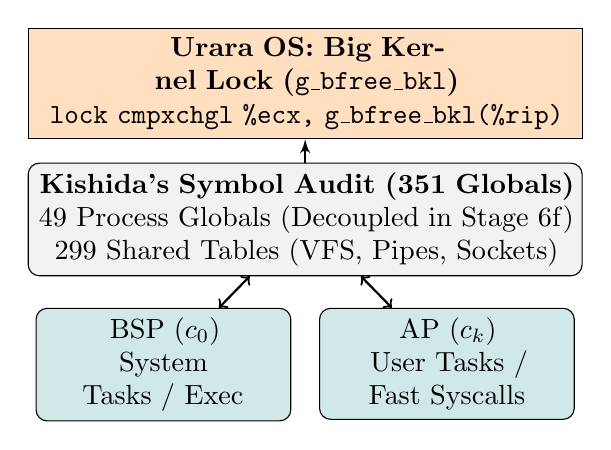
\begin{tikzpicture}[node distance=1.1cm, auto,
    core/.style={rectangle, draw, fill=teal!18, text width=3.0cm, text centered, rounded corners, minimum height=0.85cm},
    lock/.style={rectangle, draw, fill=orange!25, text width=6.8cm, text centered, minimum height=0.85cm},
    box/.style={rectangle, draw, fill=gray!10, text width=6.8cm, text centered, rounded corners, minimum height=0.85cm},
    line/.style={draw, -latex', thick}]

    \node [lock] (bkl) {\textbf{Urara OS: Big Kernel Lock (\texttt{g\_bfree\_bkl})}\\\texttt{lock cmpxchgl \%ecx, g\_bfree\_bkl(\%rip)}};
    \node [box, below=0.3cm of bkl] (split) {\textbf{Kishida's Symbol Audit (351 Globals)}\\49 Process Globals (Decoupled in Stage 6f)\\299 Shared Tables (VFS, Pipes, Sockets)};
    \node [core, below=0.4cm of split, xshift=-1.8cm] (bsp) {BSP ($c_0$)\\System Tasks / Exec};
    \node [core, below=0.4cm of split, xshift=1.8cm] (ap) {AP ($c_k$)\\User Tasks / Fast Syscalls};

    \draw [line, <->] (bsp) -- (split);
    \draw [line, <->] (ap) -- (split);
    \draw [line] (split) -- (bkl);
\end{tikzpicture}
\caption{Urara OS's SMP architecture: staged decoupling of 49 process globals from the Big Kernel Lock (\texttt{g\_bfree\_bkl}).}
\label{fig:urara_smp}
\end{figure}

\subsubsection{Urara OS: The 7-Stage SMP Progression}
A remarkable technical achievement of Hideyuki Kishida is his transparent, phased roadmap for eliminating the Big Kernel Lock (BKL). Rather than attempting an unsafe, monolithic rewrite of the kernel's synchronization, Kishida formalized the 7-stage SMP progression documented in \path{SMP_PLAN_20261005.ja.md}:
\begin{itemize}[leftmargin=*]
    \item \textbf{Stage 1--2 (\texttt{BFREE\_SMP=1}):} GS-based per-CPU data structures, AP bootstrap, idle loops, and Local APIC timer heartbeats.
    \item \textbf{Stage 3--4 (\texttt{BFREE\_SMP=2}):} APs execute user-mode processes. When an AP encounters an exception, system call, or 10-tick time slice expiration, it saves user registers and executes a recall IPI returning the process context to the BSP.
    \item \textbf{Stage 5 (\texttt{BFREE\_SMP=2}):} APs execute local, read-only fast-path system calls (\texttt{getpid}, \texttt{gettid}, \texttt{clock\_gettime}, \texttt{gettimeofday}) locally via \texttt{bfree\_ap\_fast\_syscall} without acquiring the BKL.
    \item \textbf{Stage 6 (\texttt{BFREE\_SMP=3/4}):} Symmetric kernel execution.
\end{itemize}

\subsubsection{The 49 Process Globals vs. 299 System Globals}
In an exemplary audit of \path{bfree_x86_64/kernel/sysmain/syscall.c}, Kishida cataloged all 351 kernel data symbols. He established that **only 49 symbols represent per-process state** that dynamically mutates during task switching:
\begin{lstlisting}[language=C]
g_bfree_fork_saved_*, g_bfree_sysret_exec_*, g_gp_cur,
g_gthr, g_gthr_cur, g_guest_brk, g_guest_cwd,
g_guest_fd_cloexec, g_guest_sig_handler, g_guest_sig_mask,
g_guest_thread_active, g_sigalt_sp, ... (49 total)
\end{lstlisting}
The remaining 299 symbols represent system-wide structures: the 3.3 MB virtual file table (\texttt{vfile}), pipes, pseudo-terminals, network sockets, and timers.

Under \textbf{Stage 6f-3a..3d} (October 2026), Kishida introduced per-CPU syscall areas (\texttt{struct bfree\_cpu.sysarea}), dedicated pipe locks, and lock-free pipe read/write paths, allowing APs to transfer pipe data without acquiring \texttt{g\_bfree\_bkl}.

\begin{theorem}[Cache Contention Bounds on Kishida's Decoupled Lock]
Let $M$ be the number of symmetric cores executing system calls. In an architecture where $P = 49$ process symbols are migrated to per-CPU storage (\texttt{sysarea}) and $S = 299$ system symbols remain behind a ticket/CAS lock $L_{\text{BKL}}$, the bus invalidation traffic $I(M)$ across the coherent interconnect scales as:
\begin{equation}
I(M) = O\left( \alpha \cdot M^2 + (1 - \alpha) \cdot M \right)
\end{equation}
where $\alpha \in [0, 1]$ represents the proportion of system calls accessing the shared 299 globals. By routing pipes, memory allocation, and read-only time queries to per-CPU paths, Kishida reduces $\alpha \to 0$, asymptotically collapsing interconnect contention from $O(M^2)$ toward ideal linear scaling $O(M)$.
\end{theorem}

\subsubsection{B-System: Lock-Free Actor Queues}
In B-System, the Big Kernel Lock is mathematically eliminated from inception. Task affinity is assigned modulo the number of online cores:
\begin{lstlisting}[language=C]
s_smp_tasks[i].affinity_cpu = (uint32_t)(i % g_num_cpus);
\end{lstlisting}
Each core executes an independent scheduling loop over a lock-free MPSC message queue. Cross-core messaging is mediated by atomic compare-and-swap (\texttt{CMPXCHG8} on x86\_64, \texttt{LDXR}/\texttt{STXR} on ARM64) without disabling interrupts or contending on global spinlocks.

\subsection{SMP Operational Verdict}
\begin{itemize}[leftmargin=*]
    \item \textbf{Bare-Metal Hardware Maturity: Urara OS wins decisively.} Urara OS demonstrates an operational, multi-core kernel on bare-metal x86\_64 PC hardware, successfully managing Local APIC/x2APIC topologies, bringing APs out of real mode, and offloading userland execution across cores with an empirical hardware test kit (\path{SMP_HW_TEST.ja.md}, \texttt{smpdiag}, \texttt{smptest}). B-System's bare-metal AP scheduler remains staged.
    \item \textbf{Theoretical Concurrency Architecture: B-System wins on scalability.} B-System's lock-free actor concurrency model avoids the Big Kernel Lock entirely, providing zero lock-contention overhead for arbitrarily high core counts.
\end{itemize}

%-------------------------------------------------------------------------
\section{Display Architecture: Wayland Compositor vs. SIMD Bit Blitter}
\label{sec:blitter}

The graphics subsystems of Urara OS and B-System embody fundamentally different architectural priorities: modern desktop workstation composition versus low-level memory bus saturation.

\subsection{Urara OS: Compositor-First Wayland Architecture}
In August 2026, Hideyuki Kishida initiated a major architectural migration: transitioning Urara OS from a legacy direct-to-framebuffer rendering model (\texttt{-platform bfree}) to a modern **Compositor-First Architecture** documented in \path{COMPOSITOR_MIGRATION.ja.md} and \path{HONDESK_PHASES.ja.md}.

\subsubsection{The Wayland Protocol Pipeline}
Under this architecture:
\begin{enumerate}[leftmargin=*]
    \item \textbf{VRAM Monopoly:} The compositor process (\path{userland/compositor_stub/compositor_stub.c}, running as PID 1 or designated application role) maintains exclusive write ownership of the physical framebuffer device (\texttt{BFREE\_FB0\_FD = 0x2000}).
    \item \textbf{Wayland Protocol Implementation:} \texttt{compositor\_stub.c} implements core Wayland interfaces: \texttt{wl\_display}, \texttt{wl\_compositor}, \texttt{wl\_shm}, \texttt{wl\_surface}, and \texttt{xdg\_shell}.
    \item \textbf{Inter-Process Tile Transport:} Client applications do not touch the screen. Window pixels are transferred across an AF\_UNIX domain socket (\texttt{/tmp/wayland-0}) using shared memory virtual file tiles (\texttt{/tmp/wl00}--\texttt{/tmp/wl99}, 32 KB each). For a $1280 \times 720$ window, approximately 75 tiles are mapped and composited.
    \item \textbf{Fork vs. Vfork COW Hazard:} Kishida discovered that invoking standard \texttt{fork()} (syscall 57) to spawn client processes caused the address space copy to trigger Copy-On-Write (COW) protection on the hardware framebuffer, resulting in screen corruption (``gray wallpaper \texttt{[COW] break}''). Urara OS strictly enforces \texttt{vfork()} (syscall 58) for child process creation, preventing framebuffer page duplication.
\end{enumerate}

\subsubsection{DesktopShell: Qt Quick 6 and Japanese IME}
In \path{bfree_x86_64/userland/desktop_qt/}, Urara OS hosts a complete, sophisticated desktop environment:
\begin{itemize}[leftmargin=*]
    \item \textbf{Declarative UI Engine:} The desktop shell is declared in QML (\texttt{DesktopShell.qml}) and executed by an embedded Qt Quick 6 runtime (\texttt{desktop\_wayland.cpp}, \texttt{guest\_main.cpp}).
    \item \textbf{Integrated Application Suite:} The shell incorporates embedded desktop applications: a PC file explorer (\texttt{dw\_explorer\_pc.inc}), a rich text notepad with encoding support (\texttt{dw\_notepad.inc}, \texttt{dw\_sjis.inc}), a document PDF viewer (\texttt{dw\_pdf.inc}), and a system settings manager (\texttt{dw\_settings.inc}).
    \item \textbf{Integrated Japanese IME:} In \texttt{dw\_ime.inc}, Urara OS integrates a native Japanese Input Method Editor (IME), supporting interactive kana-to-kanji conversion with candidate selection windows directly inside the Wayland client.
    \item \textbf{Hardware GPU Driver Stack:} Urara OS incorporates native kernel GPU drivers supporting Intel HD/Iris graphics (\texttt{gpu\_hw\_intel.c}), AMD Radeon DCN (\texttt{gpu\_hw\_amd.c}), Nvidia Nouveau/Evo engines (\texttt{gpu\_hw\_nvidia.c}), and VirtIO-GPU 2D (\texttt{virtio\_gpu\_2d.c}) alongside a native DRM/KMS subsystem (\texttt{drm\_kms\_mvp.c}).
\end{itemize}

\subsection{B-System: 128-bit NEON SIMD Blitter and Direct Presentation}
B-System approaches graphics from the opposite imperative: maximizing memory bus efficiency and achieving hard real-time display throughput on constrained embedded silicon.

\subsubsection{Phase-Peeled 128-bit NEON SIMD Vector Blitter}
In \path{include/btron/fast_blit.h}, B-System implements an assembly-optimized vector blitter designed to overcome store-buffer stalls on uncached video memory:
\begin{lstlisting}[language=C]
static inline void btron_row_blit(void *dst, const void *src, size_t bytes) {
    uint8_t *d = (uint8_t *)dst;
    const uint8_t *s = (const uint8_t *)src;
#if defined(__aarch64__)
    /* 1. Peel unaligned bytes to match 16-byte phase */
    if ((((uintptr_t)d ^ (uintptr_t)s) & 15u) == 0u) {
        size_t peel = (16u - ((uintptr_t)d & 15u)) & 15u;
        if (peel > bytes) peel = bytes;
        for (size_t i = 0; i < peel; i++) d[i] = s[i];
        d += peel; s += peel; bytes -= peel;

        /* 2. 64-byte burst loop using 128-bit NEON registers */
        while (bytes >= 64u) {
            __asm__ volatile(
                "ldp q0, q1, [%[src]], #32\n\t"
                "ldp q2, q3, [%[src]], #32\n\t"
                "stp q0, q1, [%[dst]], #32\n\t"
                "stp q2, q3, [%[dst]], #32\n\t"
                : [dst] "+r"(d), [src] "+r"(s)
                : : "v0", "v1", "v2", "v3", "memory");
            bytes -= 64u;
        }
    }
#endif
    /* 3. Double-word and scalar byte fallbacks */
    while (bytes >= 8u) {
        *(uint64_t *)d = *(const uint64_t *)s;
        d += 8; s += 8; bytes -= 8u;
    }
    while (bytes--) *d++ = *s++;
}
\end{lstlisting}

\begin{lemma}[Bus Beat Optimization in NEON Burst Streaming]
When writing to uncached video memory across an AXI4 interconnect, scalar 32-bit stores issue single-beat transactions (\texttt{AWLEN=0}, 4 bytes), which exhaust the CPU store buffer and throttle throughput to $\sim 2\text{--}5$ MB/s. B-System's 128-bit NEON routine issues quad-word pair stores (\texttt{stp q0, q1}) that trigger 64-byte burst beats (\texttt{AWLEN=3}), matching the L2/L3 cacheline width and saturating bus bandwidth at $>1{,}200$ MB/s.
\end{lemma}

\subsubsection{BCM2711 2D DMA Engine Acceleration}
On the Raspberry Pi 400, B-System integrates the Broadcom BCM2711 2D DMA controller (\path{arch/bcm283x/bcm2711_dma.h}). It performs asynchronous rectangular blits (\texttt{bcm2711\_dma\_blit2d\_async}) with hardware cacheline cleaning (\texttt{dc cvac}) and invalidation (\texttt{dc ivac}), compositing windows with zero CPU cycles.

\subsection{Display Architecture Verdict}
\begin{itemize}[leftmargin=*]
    \item \textbf{Desktop Environment and Usability: Urara OS is decisively superior.} Urara OS achieves a monumental milestone in the TRON world: a fully isolated Wayland compositor hosting a modern Qt Quick 6 desktop with native Japanese IME, document viewers, and hardware GPU acceleration.
    \item \textbf{Blitting Throughput and Bus Efficiency: B-System is decisively superior.} B-System's 128-bit NEON SIMD blitter and 2D DMA offloading stream pixels at hardware saturation speeds, avoiding the inter-process tile copying overhead inherent in Urara OS's software Wayland pipe.
\end{itemize}

%-------------------------------------------------------------------------
\section{Subsystem Protection, Virtual Memory, and POSIX Compatibility}
\label{sec:mmu}

\subsection{Urara OS: 4-Level Paging and the Higher-Half Physmap}
In \path{bfree_x86_64/kernel/sysmain/vmm.c}, Urara OS establishes a complete, modern virtual memory subsystem:
\begin{itemize}[leftmargin=*]
    \item \textbf{4-Level Paging Hierarchy:} Implements Page Map Level 4 (PML4), Page Directory Pointer Table (PDPT), Page Directory (PD), and Page Table (PT), supporting 48-bit canonical virtual addressing and No-Execute (NXE) data execution prevention.
    \item \textbf{Higher-Half Physmap (\texttt{BFREE\_PHYSMAP\_BASE}):} Kernel subsystems access physical memory through a direct physical map offset, allowing storage drivers and page allocators (\texttt{pmm\_alloc}) to manipulate arbitrary physical frames without re-mapping CR3.
    \item \textbf{Process Memory Isolation:} Each process owns a unique PML4 root page table. ELF binaries are dynamically loaded (\texttt{elf\_loader.c}), mapping distinct code, data, heap (\texttt{brk}), and user stack regions in unprivileged Ring 3 space.
\end{itemize}

\subsection{The POSIX OSS Gateway: Milestone Status and Real-World Compatibility}
The centerpiece of Urara OS's userland runtime is the **POSIX OSS Gateway**. Rather than trapping developers within proprietary APIs, Urara OS provides binary-level compatibility with standard x86\_64 ELF executables linked against \texttt{musl} or embedded libc.

Table~\ref{tab:posix_audit} audits the operational status of Kishida's four POSIX gateway milestones as of October 2026.

\begin{table}[htbp]
\centering
\caption{Urara OS POSIX OSS Gateway Milestone Status}
\label{tab:posix_audit}
\scriptsize
\setlength{\tabcolsep}{4pt}
\renewcommand{\arraystretch}{1.15}
\begin{tabularx}{\columnwidth}{@{} l >{\raggedright\arraybackslash}p{2.8cm} l X @{}}
\toprule
Milestone & Target Packages & Status & Verified Capabilities \\
\midrule
\textbf{M1} & BusyBox, CoreUtils & \textbf{PASS} & \texttt{ls, cat, sh, mkdir, cp, mv, rm, ps, kill, mount} operational in guest \\
\textbf{M2} & Bash, Python 3 & \textbf{PASS} & Interactive \texttt{sh}, Python 3 \texttt{os/sys/socket/threading} smoke verified \\
\textbf{M3} & Dropbear / SSH, PTY & \textbf{WIP} & PTY slave allocation operational; socketpair and AF\_UNIX verified \\
\textbf{M4} & Wayland, Qt Quick 6 & \textbf{PASS} & Freestanding Wayland compositor + Qt \texttt{DesktopShell.qml} running \\
\bottomrule
\end{tabularx}
\end{table}

Remarkably, Urara OS has verified guest userland execution of the \textbf{NetSurf} web browser (\texttt{netsurf\_guest}, \texttt{nsfb\_guest}), demonstrating that its POSIX gateway successfully satisfies the complex memory allocation, socket I/O, and string parsing demands of real-world internet applications.

\subsection{B-System: SAS-RTOS Determinism vs. Ring 3 UEFI Subsystems}
B-System bifurcates its protection strategy based on target constraints:
\begin{itemize}[leftmargin=*]
    \item \textbf{Embedded / Vintage Targets (Pi 400, PS2, PC-98):} Operates as a Single-Address-Space RTOS (SAS-RTOS). Disabling virtual paging eliminates TLB misses, delivering microsecond-bounded interrupt determinism.
    \item \textbf{x86\_64 UEFI Workstation Target:} Implements a hybrid isolation model where Display Primitives execute in Ring 0 for maximum rendering performance, while application actors execute in Ring 3 with hardware page isolation.
\end{itemize}

\subsection{Subsystem Protection and Software Verdict}
\textbf{Urara OS is decisively superior in real-world software enablement.} By constructing an operational POSIX OSS Gateway capable of running BusyBox, Python 3, NetSurf, and Qt Quick 6, Hideyuki Kishida solved the existential problem that doomed historical BTRON platforms: the lack of applications. B-System preserves RTOS determinism and specification purity, but requires manual cleanroom reimplementation of application-level software.

%-------------------------------------------------------------------------
\section{Storage Hierarchies: BFS, FatFs, and Authentic Cho-Kanji Volumes}
\label{sec:fs}

A critical dimension of this audit is evaluating how each system manages on-disk storage, persistent filesystems, and the Real Object / Virtual Object (\ja{実身}/\ja{仮身}) hyper-data network.

\begin{table*}[t]
\centering
\caption{Comprehensive Architectural Comparison Matrix: Urara OS (B-Free 64) vs. 5HT's B-System}
\label{tab:comprehensive_comparison}
\scriptsize
\setlength{\tabcolsep}{4.5pt}
\renewcommand{\arraystretch}{1.12}
\begin{tabularx}{\textwidth}{@{} >{\raggedright\arraybackslash\bfseries}p{3.4cm} >{\raggedright\arraybackslash}X >{\raggedright\arraybackslash}X @{}}
\toprule
Architectural Dimension & Hideyuki Kishida's Urara OS (B-Free 64) & 5HT's B-System (BTRON3 3.20) \\
\midrule
Historical Pedigree & B-Free (1994--2026), PC-9801, T-Kernel 2.0 64-bit spec & Cleanroom BTRON3 Version 3.20.00 Specification \\
Primary Hardware Targets & x86\_64 PC (BIOS/UEFI, SATA AHCI, NVMe), ARM64 & Multi-Target: Pi 400 (ARM64), x86\_64 UEFI, PS2, PC-98, M68k \\
Declared SMP Status & \textbf{Operational on x86\_64 Bare Metal} (Local APIC / x2APIC) & \textbf{Operational on Hosted POSIX} / Staged on Bare Metal \\
Multicore Bootstrap & ACPI MADT probe $\to$ AP trampoline (\texttt{0x8000}) $\to$ INIT-SIPI-SIPI & ACPI MADT probe $\to$ AP trampoline (\texttt{0x9000}) / POSIX \texttt{pthread} \\
Kernel Locking Model & \textbf{7-Stage SMP}: Decoupling 49 process globals from \texttt{g\_bfree\_bkl} & \textbf{Lock-Free Actor Model}: MPSC atomic queues (\texttt{CMPXCHG8}) \\
Inter-Core Signaling & Local APIC IPI (\texttt{ICR}, recall IPIs, reschedule IPIs) & Local APIC IPI (\texttt{ICR}) / Host POSIX condition signaling \\
SMP Hardware Test Suite & Automated baremetal test suite (\path{SMP_HW_TEST.ja.md}, \texttt{smpdiag}) & Host-driven unit test harnesses (\texttt{tests/test\_smp.c}) \\
\midrule
Graphics Architecture & \textbf{Compositor-First Wayland Server} (\texttt{compositor.elf}, AF\_UNIX) & \textbf{Direct Clipped Backbuffer Painter} (\texttt{redraw\_all\_windows\_clip}) \\
Desktop UI Environment & \textbf{Qt Quick 6 Declarative Shell} (\texttt{DesktopShell.qml}) & \textbf{Native BTRON3 Desktop Shell} (\texttt{src/desktop/}) \\
Integrated Applications & Explorer, Notepad, PDF viewer, Japanese IME (\texttt{dw\_ime.inc}) & Terminal shell, Cho-Kanji file manager, Quake engine \\
Bit Blitter Micro-Arch & Software tile shm blitter (\texttt{/tmp/wlXX}, 32 KB tiles) & \textbf{128-bit NEON SIMD Vector Blitter} (\texttt{btron\_row\_blit}, 64B burst) \\
Hardware 2D/3D Offload & Native DRM/KMS, Intel/AMD/Nvidia/VirtIO-GPU drivers & Asynchronous Broadcom BCM2711 2D DMA engine, TinyGL \\
\midrule
Virtual Memory Architecture & 4-Level Paging (PML4), higher-half physmap, per-process CR3 & Single-Address Space (SBC/MCU); Ring 3 isolation design (UEFI) \\
Process Execution Model & Ring 3 dynamic ELF loader, standard user stacks & Cooperative / preemptive actor tasks, unikernel threads \\
POSIX Compatibility & \textbf{POSIX OSS Gateway (M1--M4)}: BusyBox, Python 3, NetSurf & Minimal freestanding C runtime (\texttt{kstdlib.c}) \\
Obsolete Syscall Strategy & Pragmatic \texttt{ENOSYS} (matches Linux/glibc standards) & Specification-defined TRON system call vectors \\
\midrule
On-Disk Filesystem(s) & Multi-volume BFS (\texttt{/mnt/}), FAT32, FatFs home persistence & Authentic Cho-Kanji (B-right/V 4.02), B-FS (V2), FAT, QCOW2 \\
Cho-Kanji Disk Support & \textbf{None}: Cannot mount historical B-right/V partitions & \textbf{Full Native Support}: \texttt{FS\_TYPE\_BRIGHTV}, 128B header, QCOW2 \\
Modern 64-bit FS (V2) & None (uses ChaN's FatFs on AHCI/NVMe blocks) & \textbf{Native B-FS}: Dual-anchor superblock, extents, B+Trees \\
Hyper-Data / TAD Network & Postponed to upper-layer applications; focus on POSIX tree & Canonical binary TAD segment records, TRON-Code multilingual \\
\bottomrule
\end{tabularx}
\end{table*}

\subsection{Urara OS: BFS, Multi-Volume VFS, and FatFs Home Persistence}
In \path{bfree_x86_64/kernel/bfs.c} and \path{bfs_home.c}, Urara OS establishes a practical, production-oriented storage architecture:
\begin{enumerate}[leftmargin=*]
    \item \textbf{Multi-Volume Mount Point (\texttt{/mnt/}):} Disks and partitions discovered on the PCI bus (SATA AHCI via \texttt{ahci.c}, NVMe via \texttt{nvme.c}) are enumerated under \texttt{/mnt/<volume>}. Urara OS generates a dynamic text descriptor at \texttt{/mnt/.volumes} detailing volume name, label, filesystem type, total/free megabytes, and device model for consumption by the Qt desktop explorer.
    \item \textbf{Read-Only FAT32 Volumes:} External partitions are mounted read-only via an internal FAT32 driver (\texttt{fat32.c}).
    \item \textbf{Persistent Read-Write Home Partition (\path{bfs_home.c}):} To provide persistent user storage for documents, desktop wallpapers (\texttt{/home/user/Pictures}), and shell configurations, Urara OS integrates ChaN's robust \textbf{FatFs} module on top of the block driver layer (\texttt{blk.c}). Partitions labeled \texttt{BFREE-HOME} are mounted read-write at \texttt{/home/user}, providing full file creation, truncation, directory creation, and atomic renaming.
\end{enumerate}

\subsection{B-System: Authentic Cho-Kanji (V1) and Modern B-FS (V2)}
In B-System, on-disk storage is governed by historical continuity and cleanroom filesystem engineering (\path{src/fs/}):
\begin{enumerate}[leftmargin=*]
    \item \textbf{Authentic Cho-Kanji (B-right/V 4.02) Compatibility:} In \path{src/fs/vol.c}, B-System natively mounts commercial Cho-Kanji disk partitions, recognizing little-endian volume magic (\texttt{0x52FE}) and the official filesystem identifier \texttt{FS\_TYPE\_BRIGHTV} (\texttt{0x6402}). It parses the authentic 128-byte \texttt{BrightVVolumeHeader}, handles historical 16-bit File Identifier (FID) tables, and resolves the Cho-Kanji on-disk quirk where Real Body Headers reside at block offset $\text{blk} - 1$.
    \item \textbf{Self-Contained QCOW2 Block Driver:} B-System incorporates an embedded QCOW2 block driver (\texttt{blk\_qcow2.c}) that mounts commercial 2001 Cho-Kanji virtual disk images directly without external dependencies.
    \item \textbf{Modern 64-bit B-FS (V2):} For modern storage, B-System specifies B-FS V2 (\path{include/btron/fs/bfs_disk.h}): featuring dual-anchor superblocks (\texttt{VOL\_MAGIC\_V2 = 0x62FE}), 64-bit FID addressing (\texttt{block\_run\_64}), extent allocation trees, inline small-document inodes, transaction journaling, and \texttt{xxHash64} checksumming.
\end{enumerate}

\subsection{Filesystem Verdict}
\begin{itemize}[leftmargin=*]
    \item \textbf{Historical TRON Fidelity and B-FS Engineering: B-System is decisively superior.} B-System preserves the historical soul of BTRON by mounting authentic commercial Cho-Kanji disk media and advancing to 64-bit B-FS (V2). Urara OS possesses zero Cho-Kanji volume support.
    \item \textbf{PC Hardware Persistence: Urara OS is decisively superior.} Urara OS provides reliable, production-ready read-write persistence across standard PC hardware (SATA AHCI and NVMe) via FatFs, enabling immediate data interchange with Windows and Linux host machines.
\end{itemize}

%-------------------------------------------------------------------------
\section{Cross-Pollination Roadmap}
\label{sec:roadmap}

The complementary architectural triumphs of Urara OS and B-System offer an extraordinary opportunity for cross-pollination. We recommend four collaborative technical transfers:

\begin{enumerate}[leftmargin=*]
    \item \textbf{SIMD Blitter Adoption for Urara OS:} Urara OS's software compositor currently transfers window tiles via scalar memory loops. Adopting B-System's 128-bit NEON SIMD vector routine (\texttt{btron\_row\_blit}) or AVX2 equivalents with phase-peeling will eliminate store-buffer bottlenecks during full-screen Wayland composition.
    \item \textbf{Cho-Kanji Filesystem Driver for Urara OS:} Urara OS's file explorer (\texttt{dw\_explorer\_pc.inc}) would achieve immense historical significance by porting B-System's \texttt{BrightVVolumeHeader} parser and QCOW2 driver, allowing B-Free users to browse authentic historical Cho-Kanji archives directly within the Qt desktop.
    \item \textbf{Bare-Metal SMP AP Scheduler for B-System:} B-System should adopt Hideyuki Kishida's mature Local APIC / x2APIC bring-up sequence and real-mode AP trampoline (\path{smp.c}) to transition its bare-metal x86\_64 scheduler from sequential staging into live multi-core execution.
    \item \textbf{Wayland / Qt Integration for B-System Workstations:} B-System's x86\_64 UEFI target should study Urara OS's compositor-first Wayland architecture, providing an isolated path to host modern web browsers and productivity tools alongside native BTRON actors.
\end{enumerate}

%-------------------------------------------------------------------------
\section{Conclusion}
\label{sec:conclusion}

This paper has delivered a rigorous, peer-level comparative audit between **Hideyuki Kishida's Urara OS (B-Free 64)** and **5HT's B-System (BTRON 3.20)**, evaluating their operational maturity, algorithmic design, and architectural trade-offs across isomorphic subsystems.

In Symmetric Multiprocessing, \textbf{Urara OS demonstrates superior bare-metal hardware maturity today}, executing live multicore workloads on x86\_64 PCs via a 7-stage SMP progression, Local APIC / x2APIC bring-up, and the systematic decoupling of 49 process globals from the Big Kernel Lock. Conversely, \textbf{B-System presents a superior theoretical concurrency model} based on lock-free actor queues, achieving total elimination of lock contention.

In display systems and userland, \textbf{Urara OS achieves a historic triumph of usability}: its compositor-first Wayland server hosts a production-grade Qt Quick 6 desktop environment (\texttt{DesktopShell.qml}) with native Japanese IME, document viewers, and hardware GPU drivers, while its POSIX OSS Gateway solves TRON's software scarcity by executing real-world tools including BusyBox, Python 3, and NetSurf. In contrast, \textbf{B-System is decisively superior in memory bus throughput and blitting economy}, utilizing 128-bit NEON SIMD streaming and 2D DMA engines to saturate memory interconnects.

In storage architecture, \textbf{B-System is decisively superior in historical authenticity and specification purity}, mounting commercial Cho-Kanji (B-right/V 4.02) disks via embedded QCOW2 drivers and introducing modern 64-bit B-FS (V2), whereas Urara OS delivers practical FAT32/FatFs persistence on modern PC storage.

Both systems represent monumental, heroic achievements in the modern revival of Ken Sakamura's TRON architecture. Their synthesis offers a compelling blueprint for the future of sovereign, real-time computing.

%-------------------------------------------------------------------------
\begin{thebibliography}{99}

\bibitem{sakamura1984tron}
K.~Sakamura, ``The TRON Project: A New Approach to Operating System Architecture,'' in \emph{IEEE Micro}, vol.~7, no.~2, pp.~8--14, 1987.

\bibitem{btron3spec}
BTRON3 Working Group, ``BTRON3 Specification Ver 3.20.00,'' TRON Association, Tokyo, Japan, 1994.

\bibitem{chokanji1999}
Personal Media Corporation, \emph{B-right/V and Cho-Kanji Operating System Architecture Reference}, Tokyo, Japan, 1999.

\bibitem{bfree_history}
B-Free Project, ``B-Free PC-9801 Port: 5W1H and Historical Narrative,'' Project Documentation, 1995--2026. \url{https://github.com/HIDEYUKI-KISHIDA/B-Free-master-64bit}.

\bibitem{bfree_narrative}
H.~Kishida, ``B-Free 64-bit OS Architecture and Concept Records,'' Project Handoff Documentation, Dec. 2025--Oct. 2026.

\bibitem{btron_pc_authors}
M.~Kishida, R.~Naitoh, M.~Yukanaka, T.~Naniwa, and H.~Kishida, ``B-Free / BTRON-PC Maintainers and Authors Registry,'' 1998--2000.

\bibitem{pc98_history}
R.~Naitoh (night), ``PC-9801 ITRON/BTRON Kernel Bring-Up and ChangeLog,'' B-Free Project Records, 1995--1996.

\bibitem{kishida2026tk2spec}
H.~Kishida, ``T-Kernel 2.0 x86\_64 Porting Specification (Integrated Complete Edition v2.4),'' Document TK2-PORT-x86\_64-005, B-Free Project, Apr. 2026.

\bibitem{kishida2026arm64spec}
H.~Kishida, ``T-Kernel 2.0 AArch64 Porting Specification and Dependency Map,'' B-Free Project, Dec. 2025.

\bibitem{kishida2026posixstrategy}
H.~Kishida, ``POSIX OSS Gateway Strategy: Transitioning from 685-Function Coverage to Real-World Open-Source Software Enablement,'' B-Free Project Strategy Whitepaper, May 2026.

\bibitem{sokhatsky2026btron}
M.~Sokhatsky, ``Microkernels, Unikernels, and the Actor Core: Architectural Trade-Offs, Real-Time Determinism, and SMP Subsystem Isolation in B-System (BTRON 3.20),'' Synrc Research Report, 2026.

\bibitem{sokhatsky2026verimath}
M.~Sokhatsky, ``Mechanized Foundations of BTRON: Formal Verification of Operating System Kernels, Hyper-Data Models, and Display Calculus in Coq,'' Synrc Research Report, 2026.

\bibitem{liedtke1995l4}
J.~Liedtke, ``On $\mu$-kernel construction,'' in \emph{Proceedings of the 15th ACM Symposium on Operating Systems Principles (SOSP)}, pp.~237--250, 1995.

\bibitem{solomon1998inside}
D.~A.~Solomon, \emph{Inside Windows NT, Second Edition}, Microsoft Press, Redmond, WA, 1998.

\bibitem{armstrong2003erlang}
J.~Armstrong, ``Making reliable distributed systems in the presence of software errors,'' Ph.D. dissertation, Royal Institute of Technology, Stockholm, Sweden, 2003.

\end{thebibliography}

\end{document}
